\documentclass{itatnew}
\usepackage{todonotes}
\usepackage{soul}
\presetkeys{todonotes}{inline}{}
\presetkeys{todonotes}{prepend}{}
\presetkeys{todonotes}{caption=TODO}{}
\def\VH#1{\textcolor{cyan}{VH: \textit{#1}}}
\def\OP#1{\textcolor{purple}{OP: \textit{#1}}}
\def\PB#1{\textcolor{red}{PB: \textit{#1}}}
\def\todo#1{\textcolor{purple}{todo: \textit{#1}}}

\definecolor{darkgreen}{rgb}{0.0, 0.5, 0.0}
\def\OD#1{{\color{darkgreen}OD: \it #1}}
\usepackage[normalem]{ulem}
\def\ODdel#1{\bgroup\markoverwith{\textcolor{darkgreen}{\rule[0.5ex]{2pt}{1pt}}}\ULon{#1}}
%\def\OD#1{\relax} % make my comments vanish
%\def\ODdel#1{#1} % make my comments vanish


\begin{document}

\title{Recurrent Neural Networks for Dialogue State Tracking}

\author{Ondřej Plátek \and Petr Bělohlávek \and Vojtěch Hudeček  \and Filip Jurčíček}

\institute{Charles University in Prague, Faculty of Mathematics and Physics \\
\email{\{oplatek,jurcicek\}@ufal.mff.cuni.cz},\\
\email{me@petrbel.cz},\\
\email{vojta.hudecek@gmail.com},\\
\texttt{http://ufal.mff.cuni.cz/ondrej-platek}}

\maketitle              % typeset the title of the contribution

% \OP{Kde vidite problem se zalamovanim slov} \PB{predict-ing, unreal-istic, individu-ally} vec TeX nechame default


%\OP{Zitra se zeptam na emaily a zda je tam nutne mit webovku. Je povinne udat jednoho korespondencniho autora. Jelikoz z cviceni se do vysledku nedostal ani jeden model udal jsem tam sebe.} \PB{jasne, s tim neni problem, jenom abychom vedeli jak to je :) pripadne by nam mohl ufal udelat mailovky a pak mit adresu ve tvaru \{jeden, druhy, treti, ..\}@ufal.cuni.cz}\\ emaily na ufalu nedostanete - to je takovej porod - jeste vetsi nez ten clanek:)

\begin{abstract}
This paper discusses models for dialogue state tracking using recurrent neural networks (RNN).
We present experiments on the standard dialogue state tracking (DST) dataset, DSTC2~\cite{henderson2014second}.
On the one hand, RNN models became state of the art in DST,
on the other hand, most state-of-the-art models are only turn-based and require dataset-specific preprocessing (e.g. DSTC2-specific) in order to achieve state-of-the-art results.
We implemented two architectures which can be used in incremental settings and require almost no preprocessing.
We compare their performance to the benchmarks on DSTC2 and discuss their properties.
With only trivial preprocessing, the performance of our models is close to the state-of-the-art results.
\end{abstract}
%
\section{Introduction}
%
Dialogue state tracking (DST) is a standard and important task for evaluating conversational agents~\cite{williams2013dialog, henderson2014second, henderson2014third}.
A dialogue state tracker summarizes the hidden information state (HIS)\cite{young2010hidden} of a user's goal from the conversation history.
User's goals are expressed in a~formal language, typically represented as a dialogue act item (DAI). 
It was shown that with a better dialogue state tracking of HIS, conversation agents achieve better success rate in overall completion of the their task~\cite{jurvcivcek2012reinforcement}.
Dialogue state tracking translates ambiguous natural language into a formal language convenient for reasoning and accessing external knowledge. Reasoning as well as the use of external knowledge are crucial to a successful conversation in a task oriented dialogue.



In our experiments, we predict the dialogue state only from ASR transcriptions of the conversation history and a word feature which fires if a word may be a property from the database.
We argue that using only database values instead of the full ontology is not only simpler but also more natural because the system can inform the users only about the values in the database.
Note that a database of information e.g., about Cambridge restaurants, naturally defines the task of the conversation by listing the information which the system can provide.
On the other hand, the domain ontology needs to be handcrafted because it defines the task by listing all the information which users can ask about.
% TODO In addition, we show in Section~\ref{sec:eval} that we achieve strong performance.\OD{Tahle věta tady trochu vlaje ve větru, nešlo by ji nějak víc propojit s předch. textem?}

In our experiments, we focus only on the {\it goal} slot predictions because the other groups are trivial to predict\footnote{The slots {\it Requested} and {\it Method} have accuracies 0.95 and 0.95 on the test set according to the state-of-the-art~\cite{williams2014web}.}.

We also experiment with another re-splitting of the DSTC2 data because there are considerable differences between the standard train and test data sets.
The DSTC2 test set was collected from different systems~\cite{henderson2014second}.
Since the data of training, development and test set are distributed differently, the resulting performance difference between training and test data is rather high.
Our experiments show that one can obtain better results by splitting the data randomly.
As a result, we conclude that DSTC2 might suggest too pessimistic view of the state-of-the-art methods in dialogue state tracking caused by the data distribution mismatch.

Our contribution is threefold. 
First, in Section~\ref{sec:model} we compare two different architectures using RNN for dialogue state tracking.
Secondly, in~Section~\ref{sec:eval} we describe state-of-the art word-by-word dialogue state trackers architectures and propose a new encoder-decoder architecture for the DST task.
Finally, in~Section~\ref{sec:eval} we show that obtaining excellent results on DSTC2 dataset is very demanding because of the training and test set dissimilarity. In contrast, we obtained much better results just by re-splitting the DSTC2 data randomly.
% TODO consider \OD{Tenhle odstavec mi přijde jako víc high-level popis toho, co děláte, možná bych ho dal před ty konkrétnější popisky (a sem jen nějaký ten obyč rozcestník)?}
% TODO measure significance and report significant improvement

\section{Dialogue state tracking on DSTC2 dataset}
Dialogue state tracking is task which updates distribution of representation of dialogue history.
In the DSTC2 dataset, the history is captured by dialogue act items and their probabilities.
A Dialogue act item is a triple of the following form $(actionType, slotName, slotValue)$.

The DSTC2 is a standard dataset for DST, and most of state-of-the-art systems in DST have reported their performance on~this dataset~\cite{henderson2014second}. 
The full dataset is freely available since January 2014 and contains 1612 dialogues in the training set, 506 dialogues in the development set and 1117 dialogues in the test set.
The conversations are annotated at the turn level where the hidden information state was annotated manually in form of $(actionType, slotName, slotValue)$ according to the domain ontology.
The task of the domain is defined by a~database of restaurants and their properties\footnote{There are six columns in the database: name, food, price\_range, area, telephone, address.}.
The~manually designed ontology which captures a~restaurant domain is also distributed with the dataset.

\section{Models}
\label{sec:model}

Our models are all based on a recurrent neural network (RNN) encoder~\cite{werbos1990backpropagation}. Similarly to RNN encoder of~\cite{zilka2015incremental}, the models update their hidden states $h$ after processing each word. The RNN encoder takes as inputs the previous state $h_{t-1}$ representing history for first $t-1$ words and features $X_t$ for the current word $w_t$. It outputs state $h_t$ representing the whole history up to current word.
We uses a~GRU cell~\cite{cho2014gru} as the update function and we learn its parameters during training.

For each input token, our RNN encoder reads the word embedding~\cite{bengio2003neural} of this token along with several binary features. 
The binary features for each word are:
\begin{itemize}
	\item the speaker role, representing either user or system,
    \item and also indicators describing whether the word is part of some named entity representing a value from the database.
\end{itemize}
  
Since DSTC2 database is a simple table with six columns, we introduce six binary features firing if the word is a substring of named entity at given column.
For example, the word {\it indian} will not only trigger the feature for column $food$ and its value {\it indian} but also for column restaurant $name$ and its value {\it indian heaven}.

Our model variants differ only in the way they predict {\it goal} labels, i.e. $food$, $area$ and $price range$, from the RNN's last encoded state.
% The first model predicts the triples of slot values $(food, area, price range)$ jointly from the encoder hidden state $h$.
The first model predicts the output slot labels independently by employing three independent classifiers (see Section~\ref{sec:indep})
The second model uses a decoder in order to predict values one after each other from the $h_{T}$ (see Section~\ref{sec:encdec}).
% We also experimented with single classifier which predicts the labels jointly (see Figure~\ref{fig_encjoint}, but it suffers from data sparsity of the predicted tuples, so we focused only on the independent label prediction and encoder-decoder models.
We also experimented with single classifier which predicts the labels jointly (see Figure~1, but it suffers from data sparsity of the predicted tuples, so we focused only on the independent label prediction and encoder-decoder models.

The models were implemented using TensorFlow~\cite{abaditensorflow} framework. By introducing more and more complex models, we aim to overcome the data sparsity problem and incorrect independence assumptions.

% \subsection{Predicting labels jointly}
% \label{sec:joint}
% The Joint model uses a single classifier to predict a tuple of slots (see Figure~\ref{fig_encjoint}).
% The model is easy to implement and it optimizes directly the evaluation metric\OD{(see sekce s evaluací?)} \ODdel{of predicting the labels jointly.}
% However, with \OD{an} increasing number of slots\OD{,} the model suffers from the curse of dimensionality and therefore\OD{,} it is not convenient for small datasets.\OD{tohle bych asi nějak rozvedl, nebo fakt vyhodil}
\begin{figure}
% 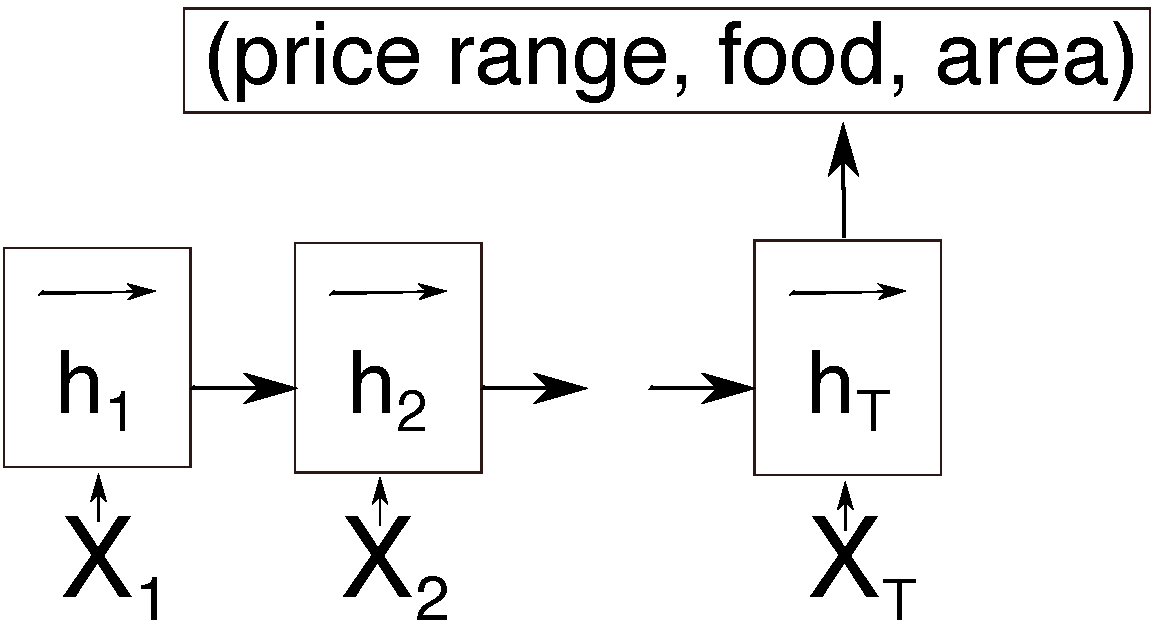
\includegraphics[width=0.5\textwidth]{encoder_joint}
\begin{center}
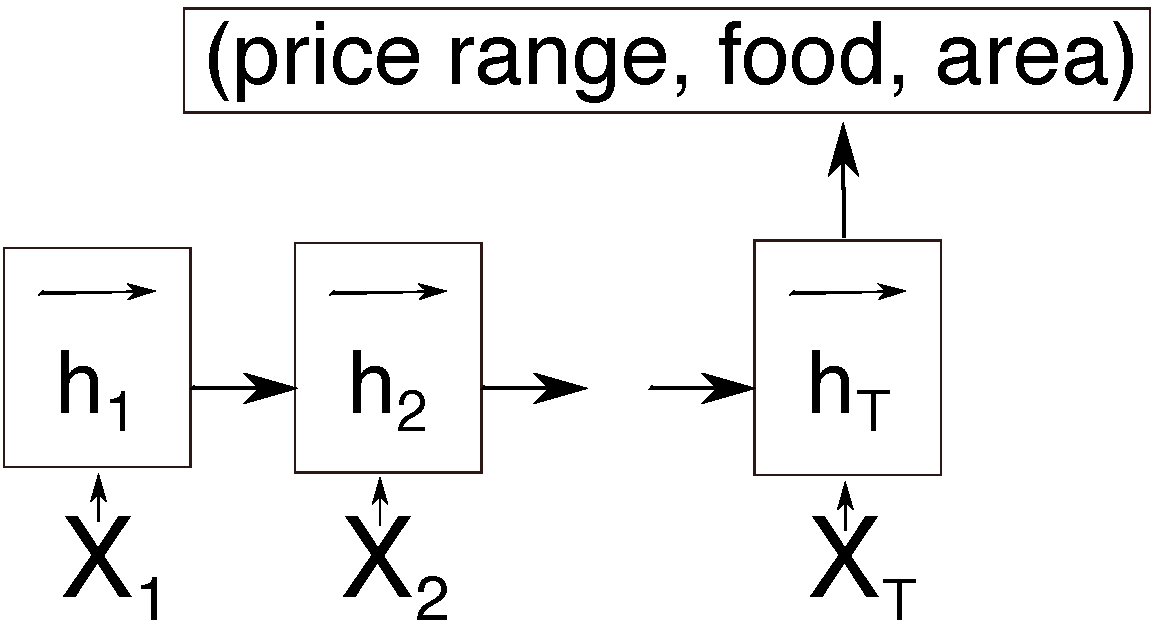
\includegraphics[height=9em]{encoder_joint}
\caption{The joint label predictions using RNN from last hidden state $h_T$. The $h_T$ represents the whole dialog history of $T$ words. The RNN takes as input for each word $i$ an embedding and binary features concatenated to~vector~$X_{i}$.}
\end{center}
\vspace{-0.70em}
\label{fig_encjoint}
\end{figure}

\subsection{Independent classifiers for each label}
\label{sec:indep}
The independent model predicts slots $food$, $area$ and $price range$ based on the last hidden state $h_{T}$ independently using three classifiers.
 % proc \OD{are} ??!!
Independent slots prediction using one classifier per each slot is straightforward to implement, but the model introduces an unrealistic assumption of uncorrelated slot properties.
In case of DSTC2 and the Cambridge restaurant domain, it is hard to believe that, e.g., the slots $area$ and $price range$ are not correlated.

\begin{figure}
\begin{center}
\includegraphics[height=9.5em]{encoder}
% \includegraphics[width=0.5\textwidth]{encoder}
\caption{The RNN encodes the word history into dialogue state $h_T$ and predicts slot values independently.}
\end{center}
\vspace{-0.80em}
\label{fig:encind}
\end{figure}

\subsection{Encoder-decoder framework}
\label{sec:encdec}
The encoder-decoder model with attention~\cite{bahdanau2014neural} is the most sophisticated model that we used for slot predictions.
To our knowledge, we are first who used this model for the task of slot predictions.
% TODO reduce space elsewhere \OD{a tady by mělo následovat povídání o tom, že vezme ten stav a token po tokenu generuje výstup USED for sequence-to-sequence problems}
The model is successfully used in machine translation where it is able to handle long sequences with good accuracy.
In DST, it captures correlation between the decoded slots easily~\cite{bahdanau2014neural}. 

The disadvantage of this model is its complexity.
Firstly, the model is not trivial to implement\footnote{We modified code from the TensorFlow `seq2seq` module.}. Secondly, the decoding time is quadratic in the length of the decoded sequences.
However, it is trivial to cast DST as a sequence-to-sequence problem. Given the dialogue history as the input sequence, we trained the model to predict a sequence of four tokens representing the first, the second, the third slot and the~end-of-string symbol.
Since our target sequence is always of length four, the model does not suffer from long decoding time. 
%\PB{In contrast, the decoding consumes asymptotically constant time regardless the input.}  to mi prijde zbytecny, to ocekavas.
\begin{figure}
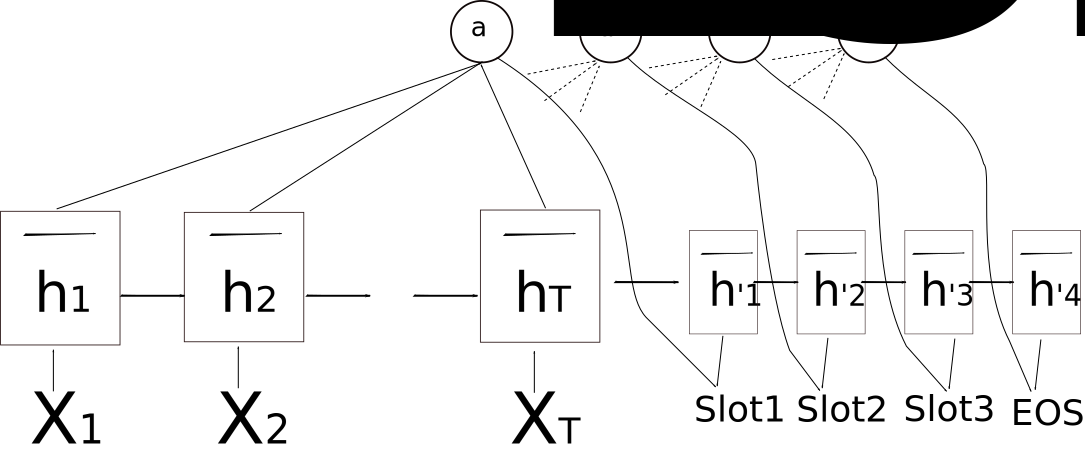
\includegraphics[width=0.5\textwidth]{encdec}
\caption{Encoder decoder with attention predicts goals.}
\label{fig:encdec}
\end{figure}

\section{Experiments}
\label{sec:exp}
We report results on the standard DSTC2 data split where we used 516 dialogues as a validation set for early stopping~\cite{prechelt1998early} and the remaining 1612 dialogues for training.
We use 1-best ASR transcriptions on the input and measure joint slot accuracy.
% For the results on the standard split of DSTC2, see~Table~\ref{tab:dstc}.
For the results on the standard split of DSTC2, see~Table~1.
We also evaluated the models on a randomly split DSTC2 dataset\, and the details are described in Section~\ref{sec:split}.


% Note that we measure accuracy with schedule 2 which skips the first turns where the believe tracker does not track any values. We use the official evaluation scripts in our experiments.
Note that we measure accuracy without schedule 2 which skips the first turns where the believe tracker does not track any values. As a consequence, we do not evaluate the models according any  standard metric.\footnote{We plan to submit the camera ready version of this article with results evaluated using the standard scripts for measuring accuracy with schedule 2.}

% \TODO{nechceme reportovat i train a valid? me to vetsinou v clancich zajima} muzem kdyz to stihnem, ale validace na trenovani trva dlouho a nechce se mi to prepocitavat na validacni sade to mame

For all our experiments, we train word embeddings of size 100 and use the encoder state size of size 100, together with a dropout keep probability of $0.7$ for both encoder inputs and outputs.
These parameters where selected by a grid search over the hyper-parameters on development data.

\subsection{Training}
\label{sec:train}
% TODO describe vocabularies and shared embeddings for encoder-decoder
The training procedure minimizes the cross-entropy loss function using the Adam optimizer~\cite{kingma2014adam} with a batch size of 10.
We train predicting goal slot values for each turn.
%An iteration which process turn $t$ uses the the whole dialogue history until the turn $t$ as an input and slot labels $labels_t$ as a reference.
We treat each dialogue turn as a separate training example, feeding the whole dialogue history up to the current turn into the encoder and predicting the slot labels for the current turn.

We use early stopping with patience~\cite{prechelt1998early}, validating on the development set after each epoch and stopping if the three top models does not change for four epochs.

The predicted labels in DST task depend not only on the last turn, but on the dialogue full history as well.
Since the lengths of dialogue histories vary a lot\footnote{The maximum dialogue history length is 487 words and 95\% percentile is 205 words for the training set.} and we batch our inputs, we separated the dialogues into ten buckets accordingly to their lengths in order to provide a computational speed-up. We reshuffle the data after each epoch only within each bucket.

In informal experiments, we tried to speed-up the training by  optimizing the parameters only on the last turn\footnote{The prediction was conditioned on the full history but we back-propagated the error only in words within the last turn.} but the performance dropped relatively by more than 40\%.

\subsection{Comparing models}
\label{sec:eval}

Predicting the labels jointly is quite challenging because the distribution of the labels is skewed as demonstrated in~Figure~\ref{fig:labels}.
% TODO novej obrazek\OD{mně z toho obrázku moc skewed nepřijde, obrázek vypadá celkem rovnoměrně, i když si nejsem jistej, co zobrazuje -- co je na tom skewed?}
Some of the labels combinations are very rare, and they occur only in the development and test set so the joint model is not able to predict them.
During first informal experiments the~joint model performed poorly arguably due to data sparsity of slot triples. We further focus on model with independent classifiers and encoder-decoder architecture.

\begin{figure}
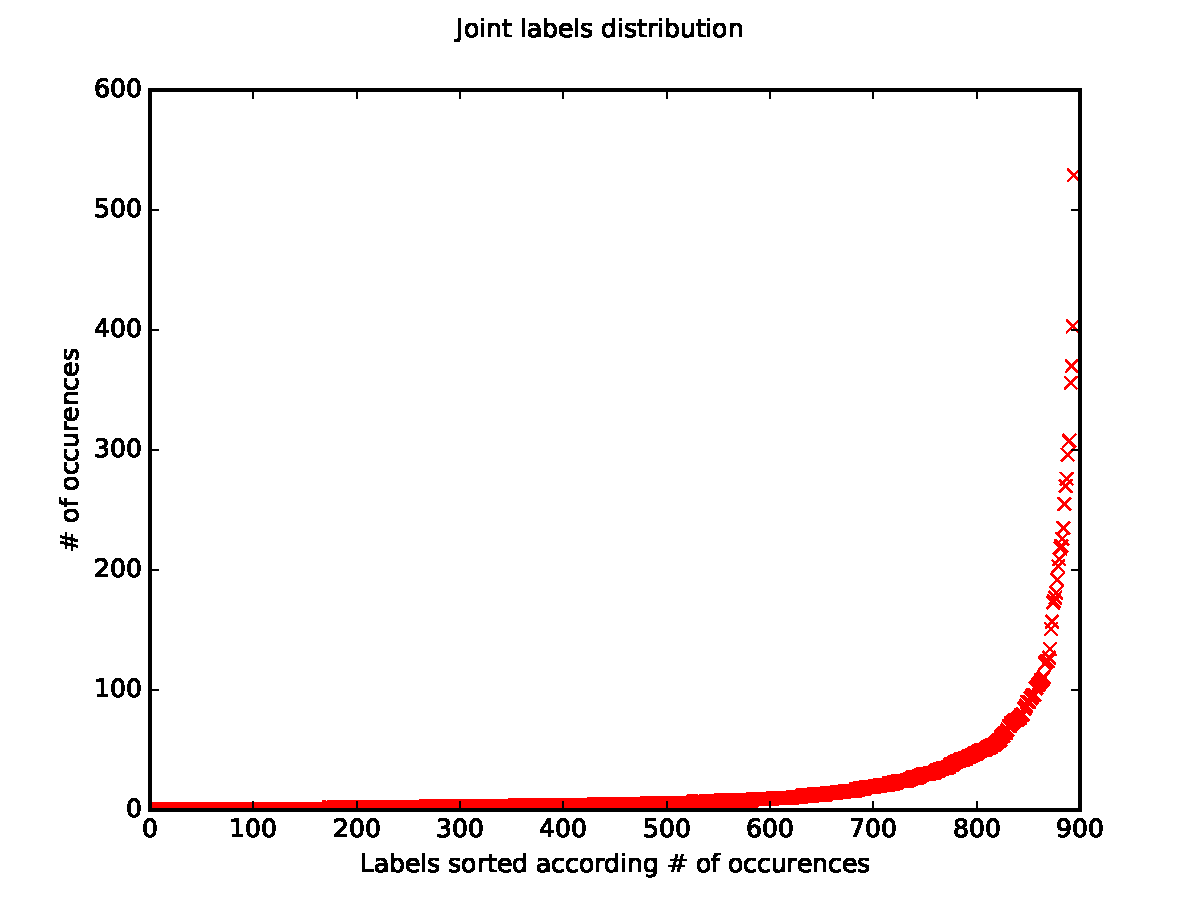
\includegraphics[width=0.5\textwidth]{jointLabelsDistrib}
\caption{The number occurrences of labels in form of $(food, area, pricerange)$ triples from the least to the most frequent.}
\label{fig:labels}
\end{figure}

% The model with independent label prediction obtained much better performance on each slot individually as expected, but also it surprisingly outperformed the joint model in the joint prediction.
% We hypothesize that with larger amount of data the joint model would suffer less from data sparsity and perform better.
% This claim is supported by comparison of joint and independent models performance on the original DSTC2 dataset.
The model with independent label prediction is a strong baseline which was used, among others, in work of~\cite{zilka2015incremental}.
The model suffers less from data set mismatch because it does not model the correlation between predicted labels.
This property can explain a smaller performance drop between the test set from reshuffled data and the official test set in comparison to encoder-decoder model.

% FIXME include results from other papers
\begin{table}
\begin{center}
\begin{tabular}{r@{\quad}rll}
\hline
\multicolumn{1}{l}{\rule{0pt}{12pt}
                   Model}&\multicolumn{1}{l}{Dev set}&\multicolumn{2}{l}{Test set}\\[2pt]
\hline\rule{0pt}{12pt}
% Joint  &  todo &  todo \\
% /a/SSD/oplatek/e2end/log/2016-06-08-17-31-38.400-dstc-INDEP_labels-d0.7-w100-e100/
% /a/SSD/oplatek/e2end/log/TEST-ORIGINAL-2016-06-08-17-31-38.400dstc-INDEP_labels-d0.7-w100-e100-reward-0.9080-step-0036224
Indep  &   0.91 & 0.76 \\
EncDec &   0.94 & 0.73 \\
\hline
\end{tabular}
\caption{Accuracy on development and test set}
\vspace{-2em}
\end{center}
\label{tab:dstc}
\end{table}


Since the encoder-decoder architecture is very general and can predict arbitrary output sequences, it also needs to learn how to predict only three slot labels in the correct order.
It turned out that the architecture learned to predict quadruples with three slot values and the end-of-string (EOS) symbol quickly, even before seeing a~half of the training data in the first epoch.
At the end of the first epoch, the system made no more mistakes on predicting slot values in the incorrect order.
The encoder-decoder system 
% TODOstrongly\OD{significance tests?/nebo: outperformed the prev. models by a wide margin?}
outperformed the previous models and the time needed for learning the output structure was surprisingly short.\footnote{The best model weights were found after 18 to 23 epochs for all model architectures.}
% TODO jak dlouho trvala epocha


\subsection{Data preparation experiments}
\label{sec:split}

% FIXME include results from other papers
\begin{table}
\begin{center}
\begin{tabular}{r@{\quad}rll}
\hline
\multicolumn{1}{l}{\rule{0pt}{12pt}
                   Model}&\multicolumn{1}{l}{Dev set}&\multicolumn{2}{l}{Test set}\\[2pt]
\hline\rule{0pt}{12pt}
% Joint  &  todo &  todo \\
Indep  &   0.87 & 0.89 \\
EncDec &   0.94 & 0.91 \\
\hline
\end{tabular}
\caption{Accuracy on the re-split DSTC2 data.}
\vspace{-2em}
\end{center}
\label{tabsplit}
\end{table}

The data for the DSTC2 test set were collected using a different spoken dialogue system configuration than the data for the validation and the training set.\cite{henderson2014second}.
We wanted to investigate how this influences the complexity of the task so we merged all DSTC2 data together and created splits of 80\%, 10\% and 10\% for the training, development and test sets.
% The~results in Table~\ref{tabsplit} show that the complexity of the task dropped significantly.
The~results in Table~2 show that the complexity of the task dropped significantly.


\section{Related work}
\label{sec:related}

There are numerous systems which reported on the DSTC2 dataset, we discuss only the systems which use RNN.
In general, the RNN systems achieved excellent results.

Our system is related to the RNN tracker of Žilka and Jurčíček~\cite{zilka2015incremental},
which reported near state-of-the art results on the~DSTC2 dataset and was the first incremental system which was able to update the dialogue state word-by-word with such accuracy.
In contrast to work of~\cite{zilka2015incremental}, we use no abstraction of slot values. Instead, we add the additional features as described in Section~\ref{sec:model}.
The first system which used a neural network for dialogue state tracking~\cite{henderson2013deep} used a feed-forward network and more than 10 manually engineered features across different levels of abstraction of the user input, including outputs of the spoken language understanding component (SLU).
In our work, we focus on simplifying the architecture, hence we used only features which were explicitly given by the dialogue history word representation and the database.

The system of Henderson et al.~\cite{henderson2014word} gives state-of-the-art results and, similarly to our system, it predicts the dialogue state from words by employing a RNN.
On the other hand, their system heavily relies on the user input abstraction.
Another dialogue state tracker with LSTM was used in reinforcement setting but the authors also used information from the SLU pipeline~\cite{lee2016dialog}.

An interesting approach is presented in the work of Vodolán et al.~\cite{vodolan2015hybrid}, who combine a rule-based and a machine learning based approach to belief state tracking.
Their work clearly separates the handcrafted features which can be easily replaced or omitted.
The features are fed to an LSTM-based RNN which performs a dialog-state update.
However, unlike our work, their system requires SLU parses on the input.

It is worth noting that there are first attempts to train an end-to-end dialogue system even without explicitly modeling the dialogue state~\cite{bordes2016learning}, which further simplifies the architecture of a dialogue system.
However, the reported end-to-end model was evaluated only on artificial dataset and cannot be compared to DSTC2 dataset directly.

\section{Conclusion}
\label{sec:conc}

We presented and compared two dialogue state tracking models which are based on state-of-the-art architectures using recurrent neural networks.
To our knowledge, we are the first to use an encoder-decoder model for the dialogue state tracking task, and we encourage others to do so because it is competative with the standard RNN model. 
Note that the standard RNN model achieves almost state-of-the-art results.

We evaluated the models on DSTC2 dataset containing task-oriented dialogues in restaurant domain. 
We trained the models using only ASR 1-best transcriptions and task-specific lexical features defined by the task database.

We also observed that obtaining high accuracy for dialogue state tracking on DSTC2 test set is notoriously hard and that the task becomes substantially easier if the data is reshuffled.

The code for our experiments is published under a permissive Apache license on Github at \url{https://github.com/oplatek/e2end/}.\footnote{Some informal experiments were conducted  within the Statistical Dialogue Systems course at Charles University in Prague and can also be  found on Github at \url{https://github.com/oplatek/sds-tracker}.}

In future work, we plan to evaluate the models using the standard DSTC2 scripts to compare them to other trackes on this dataset.
In addition, we would like to investigate how much the introduced database features improved the performance of the models.
Our future plans also concern collecting and annotating more data which would allow us to evaluate the models on another task-oriented dataset.

\subsection*{Acknowledgment}
We would like to thank Mirek Vodolán for help with evaluation scripts and Ondřej Dušek for useful comments.
This research was partly funded by the Ministry of Education, Youth and Sports of the Czech Republic under the grant agreement LK11221, core research funding, grant GAUK 1915/2015, and also partially supported by SVV project number 260 333. 
We gratefully acknowledge the support of NVIDIA Corporation with the donation of the Tesla K40c GPU used for this research.
Cloud computational resources were provided by the MetaCentrum under the program LM2010005 and the CERIT-SC under the program Centre CERIT Scientific Cloud, part of the Operational Program Research and Development for Innovations, Reg.\ no. CZ.1.05/3.2.00/08.0144.
% TODO myslim, ze to mam dobre, ale v camera ready to zkontrolujem - nestiham. \PB{nemusi byt podekovani metacentru v nejake jejich oficialni podobe - link v komentari?} %https://wiki.metacentrum.cz/wiki/Pravidla_vyu%C5%BEit%C3%AD_MetaVO/Pod%C4%9Bkov%C3%A1n%C3%AD

\newpage
\bibliographystyle{plain}
\bibliography{samplearticle}
\end{document}
